\newpage
ҒТАМР 31.15.27; 61.51.01
\hfill {\bfseries \href{https://doi.org/10.58805/kazutb.v.3.24-458}{https://doi.org/10.58805/kazutb.v.3.24-458}}

\sectionwithauthors{Е.Б. Асылбеков, С.А. Тунгатарова, G.G. Xanthopoulou, Т.С. Байжуманова, М. Жумабек}{SHS ӘДІСІМЕН СИНТЕЗДЕЛГЕН КАТАЛИЗАТОРЛАРДЫ ӘРТҮРЛІ ЖАҒДАЙДА
САЛҚЫНДАТУДЫҢ ӘСЕРІН ЗЕРТТЕУ}

\begin{center}
{\bfseries \textsuperscript{1,2}Е.Б. Асылбеков\envelope, С.А. Тунгатарова\textsuperscript{1,2}, G.G. Xanthopoulou\textsuperscript{3}, Т.С. Байжуманова\textsuperscript{1,2}, М. Жумабек\textsuperscript{1}}

\textsuperscript{1}Д.В. Сокольский атындағы отын, катализ және
электрохимия институты, Алматы, Қазақстан,

\textsuperscript{2}Әл-Фараби атындағы Қазақ ұлттық университеті, Алматы,
Қазақстан,

\textsuperscript{3}National Center for Scientific Research «Demokritos»,
Athens, Greece
\end{center}
\envelope Корреспондент-автор: yer-asyl@mail.ru


Өзін-өзі тарататын жоғары температуралы синтез (SHS) әдісі заманауи
керамика, металаралық қосылыстар, катализаторлар және магниттік заттарды
қоса алғанда, әртүрлі инженерлік және функционалды материалдардың үнемді
өндірісін жеңілдету үшін бүкіл әлемде дамып келеді. Бұл әдіс өз өзімен
жануын қолдайтын реакцияларға негізделген, олар өте қысқа мерзім ішінде
жүреді және материалдар ішіндегі өте жоғары ішкі температураға ие
болады. Демек, SHS дәстүрлі әдістерге қарағанда бірқатар артықшылықтарды
ұсынады, соның ішінде энергия шығындарын айтарлықтай азайту, қоршаған
ортаға зиян әсерін азайту, өндіріс процестерін жеңілдету және ерекше
қасиеттері мен сипаттамалары бар материалдарды жасау. Бұл мақала SНS
әдісін зерттейді, оның артықшылықтарын атап көрсетеді және сутекті
өндіру және метанолды конверсиялау үшін жоғары белсенді катализаторларды
әзірлеу сияқты бірнеше экологиялық маңызды қолданбаларды қарастырады.
Сонымен қатар, SНS қоршаған орта температурасында басталып, аяқталуы
мүмкін болғандықтан, ол улы немесе радиоактивті материалдармен және
ластанған заттармен жұмыс істеуде тиімді, бұл әдіс әйнектеу,
шоғырландыру және қауіпті қалдықтарды инкапсуляциялау арқылы кең
қорғаныс жабындарын қалыптастыруға мүмкіндік береді. Сондай-ақ, бұл әдіс
әртүрлі спирттер мен көмірсутектердің бу конверсиясының катализаторларын
синтездеуде жақсы нәтиже көрсетті.

{\bfseries Түйін сөздер:} көмірсутектер, спирттер, мыс негізіндегі
катализаторлар, SНS әдісі, сутегі.

\sectionheading{ИЗУЧЕНИЕ ЭФФЕКТА ОХЛАЖДЕНИЯ КАТАЛИЗАТОРОВ, СИНТЕЗИРОВАННЫХ
МЕТОДОМ SHS, В РАЗЛИЧНЫХ УСЛОВИЯХ}

\begin{center}
{\bfseries \textsuperscript{1,2}Е.Б. Асылбеков\envelope, \textsuperscript{1,2}С.А.
Тунгатарова, \textsuperscript{3}G.G. Xanthopoulou,}

{\bfseries \textsuperscript{1,2}Т.С. Байжуманова, \textsuperscript{1}М.
Жумабек}

\textsuperscript{1}Институт топлива, катализа и электрохимии им. Д.В.
Сокольского, Алматы, Казахстан,

\textsuperscript{2}Казахский национальный университет имени Аль-Фараби,
Алматы, Казахстан,

\textsuperscript{3}National Center for Scientific Research «Demokritos»,
Athens, Greece

e-mail: yer-asyl@mail.ru
\end{center}

Метод самораспространяющегося высокотемпературного синтеза (СВС)
развивается во всем мире, чтобы облегчить экономичное производство
различных инженерных и функциональных материалов, включая современную
керамику, интерметаллические соединения, катализаторы и магнитные
вещества. Этот метод основан на реакциях самоподдерживающегося горения,
которые за очень короткий период создают чрезвычайно высокие внутренние
температуры внутри материала. Следовательно, СВС предлагает ряд
преимуществ по сравнению с традиционными методами, включая значительное
снижение затрат на электроэнергию, снижение воздействия на окружающую
среду, упрощение производственных процессов и создание материалов с
отличительными свойствами и характеристиками. В этой статье исследуется
метод СВС, подчеркиваются его преимущества и рассматриваются несколько
экологически важных применений, таких как разработка высокоактивных
катализаторов для производства водорода и конверсии метанола. Кроме
того, поскольку СВС можно начинать и завершать при температуре
окружающей среды, он эффективен для обращения с токсичными или
радиоактивными материалами и загрязненными объектами, позволяя
формировать на месте обширные защитные покрытия или путем остекления,
консолидации и инкапсуляции опасных отходов. Также этот метод отлично
показал себя при синтезе катализаторов паровой конверсии различных
спиртов и углеводородов.

{\bfseries Ключевые слова:} углеводороды, спирты, катализаторы на основе
меди, метод СВС, водород.

\sectionheading{STUDYING THE EFFECT OF COOLING CATALYSTS SYNTHESIZED BY SHS
METHOD UNDER DIFFERENT CONDITIONS}

\begin{center}
{\bfseries \textsuperscript{1,2}Y.B. Assylbekov\envelope, \textsuperscript{1,2}S.А.
Tungatarova, \textsuperscript{3}G.G. Xanthopoulou,}

{\bfseries \textsuperscript{1,2}Т.S. Baizhumanova,
\textsuperscript{1}Zhumabek M.}

\textsuperscript{1}JSC ``D.V. Sokolsky Institute of Fuel, Catalysis and
Electrochemistry'', Almaty, Kazakhstan,

\textsuperscript{2}Al-Farabi Kazakh National University, Almaty,
Kazakhstan,

\textsuperscript{3}National Center for Scientific Research «Demokritos»,
Athens, Greece

e-mail: yer-asyl@mail.ru
\end{center}

The self-propagating high-temperature synthesis (SHS) technique is being
advanced globally to facilitate the economical production of various
engineering and functional materials, including modern ceramics,
intermetallic compounds, catalysts, and magnetic substances. This
technique relies on self-sustaining \\combustion reactions, which generate
extremely high internal temperatures within the material in a very brief
period. Consequently, SHS offers several benefits over traditional
methods, including significantly reduced energy costs, lower
environmental impact, simplified production processes, and the creation
of materials with distinctive properties and characteristics. This paper
explores the SHS method, highlighting its benefits and examining several
environmentally relevant applications, such as the development of highly
active catalysts for hydrogen production and methanol conversion.
Additionally, because SHS can be initiated and completed at ambient
temperatures, it is effective for managing toxic or radioactive
materials and contaminated sites by enabling on-site formation of
extensive protective coatings or by glazing, consolidating, and
encapsulating hazardous waste. Also, this method has shown itself to be
excellent in the synthesis of catalysts for steam reforming of various
alcohols and hydrocarbons.

{\bfseries Keywords:} hydrocarbons, alcohols, Cu-based catalysts, SHS
method, hydrogen.

\begin{multicols}{2}
{\bfseries Кіріспе.} Өзін-өзі тарататын жоғары температуралы синтез (SHS)
әдісі -- бұл бақылаулы жану синтезінің бір түрі болып таыблады және
қазір көптеген елдерде кеңінен қолданылады. Бұл салыстырмалы түрде жаңа
әдіс болғандықтан, көптеген қосымша зерттеулер мен бақылауларды талап
етеді {[}1{]}. SHS процесі өте экзотермиялық, қатты жалынды реакцияларын
пайдалана отырып, ұнтақ компоненттері арасында басқарылатын жоғары
температуралы жану арқылы көптеген бірегей материалдарды
(катализаторларды) синтездейді. Ол алғаш рет 1967 жылы бұрынғы Кеңес
Одағында жарияланды, бірақ әлемге тек 70-жылдардың басында белгілі
болды. SHS-ті қолдана отырып, материалдардың құрамы, құрылымы және
қасиеттері көптеген қолданбалар талаптарына сәйкес келетіндей етіп
реттелуі мүмкін. Жануды бастау химиялық жолмен немесе электрлік
қыздырылған элемент арқылы жүзеге асады. Жану басталғаннан кейін, ол
өзін-өзі ұстап, басталу жағынан қарама-қарсы жағына қарай сығылған
материал арқылы жану толқыны өтеді және бірнеше секундтан бірнеше
минутқа дейінгі уақытта аяқталады {[}2, 3{]}. Үлгі бөлме
температурасында немесе салыстырмалы түрде төмен температурада -- сирек
1000°C жоғары -- алдын ала қыздырылған болуы мүмкін {[}4, 5{]}. Таралып
жатқан толқынның алдындағы материал жану нәтижесінде бөлінетін жылумен
алдын ала қыздырылады, ал жану фронтының артындағы материал толқын өткен
кезде тез салқындайды. SHS процесінің схемалық диаграммасы 1-суретте
көрсетілген. SHS негізгі принциптері ретінде келесілерді айтуға болады:

\begin{itemize}
\item
  Процесс реакциялары арқылы қажетті құрам мен құрылымдағы өнімдерді тез
  автотолқындық жандыру;
\item
  Химиялық реакцияларда бөлінетін ішкі жылуды пайдалану арқылы сыртқы
  энергия көзін толық немесе ішінара жою;
\item
  Жылу бөліну және тасымалдану жылдамдығын өзгерту арқылы процестің
  жылдамдығын, температурасын, конверсия дәрежесін және өнімдердің
  құрамы мен құрылымын бақылау.
\end{itemize}
\end{multicols}

\begin{figure}[H]
	\centering
	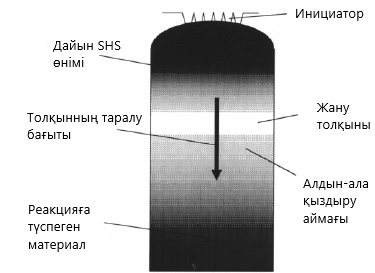
\includegraphics[width=0.4\textwidth]{assets/69}
	\caption*{1-сурет - SHS процесінің схемалық көрнекі сызбасы}
\end{figure}

\begin{multicols}{2}
Бұл принциптер дәстүрлі өңдеу әдістеріне қарағанда елеулі артықшылықтар
береді. Көптеген жағдайларда SHS дәстүрлі әдістермен салыстырғанда төмен
өндіріс шығындары және өндірістік артықшылықтармен, сондай-ақ,
микроструктура мен жоғары қасиеттерімен үлкен пайда ұсынады.

Химиялық қосылыстарды, оның ішінде органикалық қосылыстарды сутегіге
айналдыру процесі каталитикалық риформинг арқылы жүзеге асырылады. Бұл
процеске қысқаша тоқтала кететін болсақ: қазіргі таңда үш дара түрі
қолданылады -- автотермиялық риформинг, ішінара тотықтандыру және бу
риформингі әдістері.

Автотермиялық риформинг кезінде бір уақытта екі түрлі реакция {[}6{]}
қатар жүреді: эндотермиялық бу риформингі мен экзотермиялық толық тотығу
реакциясы. Соның нәтижесінде процестің энтальпиясы нөлге жақын болады
да, реакция (1) сыртқы жылу беруді қажет етпейді:

\begin{equation}
\text{4CH3OH + 3H2O + 0,5O2 = 4CO2 + 11H2}
\end{equation}
\begin{equation*}
\text{∆rH0 \textasciitilde{} 0 кДж·моль-1}
\end{equation*}

Метанолдың оттегімен ішінара тотығуы {[}7{]} экзотермиялық жолмен жүреді
және реакция (2) аймағынан бөлінетін жылуды кетіруді (бөліп шығаруды)
қажет етеді:

\begin{equation}
\text{CH3OH + 0,5O2 = CO2 + 2H2}
\end{equation}
\begin{equation*}
\text{∆rH0 = +192 кДж·моль-1}
\end{equation*}

Метанолдың булы риформингі {[}8{]} эндотермиялық реакция (3) болып
табылады және реакция аймағына жылу беруді қажет еткенімен, қолдануға
ыңғайлы және арзан әдіс болып келеді:

\begin{equation}
\text{2CH3OH + O2 = 2CO2 + 4H2}
\end{equation}
\begin{equation*}
\text{∆rH0 = -49.4 кДж·моль-1}
\end{equation*}

Ал құрамында мысы бар катализаторларды қолдану булы реформинг процесін
200-400 °C температурада жүргізуге мүмкіндік береді. Бұл жағдайда
метанолды 100\% конверсиялау үшін реактивтердің катализатор қабатымен
жанасуы ұзақтығы 0,1-1 секундтан аспайтын уақыт жиі жеткілікті болып
келеді.

Осы процеске сайма сай катализаторды SHS, яғни өздігінен таралатын
жоғары температуралы синтез әдісі бойынша дайындадық. Өздігінен
таралатын жоғары температуралық синтез (SHS) конденсацияланған
жүйелердің бақыланатын жануына негізделген. Ұнтақтардың мұқият
жобаланған және бақыланатын қоспаларының өзін-өзі қамтамасыз ететін
экзотермиялық жануы кезінде синтез температурасы реакцияның өте қысқа
болып келетін жалпы алғандағы уақытында 1500-3000°C жетуі мүмкін, яғни
бірнеше секунд ішінде ғана {[}9{]}. Бұл мезетте «жану» процесі алынған
үлгі бойымен жану толқынының таралуы түрінде жүреді. Аталған жағдайларда
синтезделген материалдар кристалдық тор ақауларының өте жоғары құрамымен
сипатталады. Бұл катализатордың белсенділігін анықтайтын өте маңызды
каталитикалық сипаттама болып табылады, өйткені олар катализ үшін
белсенді учаскелер ретінде әрекет етеді. Жану толқыны өткеннен кейін
толқындық «фронттың» артында қалған материал салқындай бастайды
{[}10{]}. Синтезделген катализатордың соңғы құрылымы мен құрамы
салқындату жылдамдығы мен сипатына байланысты өзгереді. Құрылымдық және
химиялық конверсияның бес аймағын бөлуге болады. V аймақ салқындату
аймағы болып табылады және материалдардың құрамы әлі де өзгеретіні анық.
Үлгіні әртүрлі жылдамдықтар мен шарттарда (минутына бірнеше жүзден
жүздеген мың градусқа дейін) салқындату композициялар ауқымын алуға,
сонымен қатар, тор ақауларының концентрациясын өзгертуге мүмкіндік
береді.

SHS өнімдерін термогравиметриялық талдау жану толқынының бойында
бастапқы ұнтақтардың көп жағдайда толық реакцияға түсіп үлгермейді деген
тұжырымға келтіреді. Талдаулардың қорытындылары көрсеткендей, синтез
өнімдері Al, CuCO\textsubscript{3}, MgCO\textsubscript{3}, және т.б.
сияқты ыдырау және тотығу температуралары салыстырмалы түрде алғанда
төмен (500-900°С) болып келетін қосылыстардан тұрады. Әдетте
қосылыстардың жану температурасы 1300°С-2500°С арасындағы шаманы
көрсетеді, бұл көптеген жағдайларда бастапқы ұнтақтардың реакцияға түсіп
үлгермей, толық ыдырайтынын көрсетеді {[}11{]}. Осы жаңалықтардың
нәтижесінде синтез жүргеннен кейінгі салқындату жылдамдығының өзгеруі
жану процестерінің ұзақтығы мен тереңдігінің өзгеруі нәтижесінде
катализатордың микроқұрылымы мен қасиеттерінің әртүрлі болып шығуы
белгіленді.

Бұл жағдай материалдардың каталитикалық белсенділігіне айтарлықтай әсер
етеді деп күтілді. Каталитикалық белсенділікті көрсететін SНS әдісімен
дайындалған катализаторлармен эксперименттер жүргізілді.

{\bfseries Материалдар мен әдістер.} Катализаторлар өздігінен таралатын
жоғары температуралы синтез (self-propagating high temperature synthesis
- SHS) әдісімен дайындалды. Біріншіден, катализаторды синтездеуге
арналған ұнтақтарды дайындап аламыз. Ол үшін метал күйіндегі таза
алюминий (Al) мен мыс (I) оксидінің (Cu\textsubscript{2}O) ұнтақтары
белгілі мөлшер мен қатынаста өлшеніп алынды. Содан соң өлшенген ұнтақтар
араластырылып, 50 бар қысым астында гидравликалық престің күшімен
нығыздап «таблетка» пішініне келтірдік.

Дайындалған таблетканы алдын ала 700°C температураға дейін тұрақты
қыздырып қойылған муфель пешіне енгіздік. Синтез реакциясы лезде
басталып, жүріп кетуі үшін реакцияның инициаторы ретінде 1 г таза магний
(Mg) ұнтағын таблетканың үстіне қойдық. 10 секунд өткеннен кейін синтез
магний тұтанып, синтез реакциясының инициациясы басталды. Пешке
енгізілген термопара арқылы синтез реакциясының өту температурасын
бақылап, тіркеп алдық.

Зерттеу жұмыстарының барысында жоғарыда аталған Al-Cu-O жүйелерінің
негізіндегі материалдар бірдей жағдайларда SHS-жануына ұшырады және
реакциядан кейін әртүрлі жағдайларда суытылды: пеш ішінде, ауада (бөлме
температурасында), азот (N\textsubscript{2}) қысымының астында. Осы
жағдайлардың синтезделген катализатордың құрылымы мен белсенділігіне
ықпалы алдағы уақытта метанолдың каталитикалық риформинг процесіне қалай
әсер ететіндігі бақыланды.

Каталитикалық риформингке дейінгі бастапқы қоспаны және процестен
кейінгі реакция өнімдерін талдау «Chromos GC-1000» (Ресей)
хроматографының көмегімен жүргізілді, ол саптама және капиллярлық
колонкалармен жабдықталған. Н\textsubscript{2}, О\textsubscript{2},
N\textsubscript{2}, СН\textsubscript{4},
С\textsubscript{2}Н\textsubscript{6},
С\textsubscript{2}Н\textsubscript{4},
С\textsubscript{3}-С\textsubscript{4} көмірсутектер, СО және
СО\textsubscript{2} талдау үшін оралған баған қолданылады.

Катализаторларды синтездеу және оларға физика-химиялық зерттеулер
«Демокритос» Ұлттық Ғылыми-Зерттеу Орталығының (Афины қ., Греция)
жетілдірілген керамика және композиттер зертханасында жүргізілді.
Синтезделген катализаторлар ішкі стандарты ретінде 10\% KCl және CuKa1
сәулеленуін қолданатын жартылай сандық Siemens Spellman DF3
спектрометрінде рентгендік дифракция (XRD) талдаулары жүргізілді.
Катализаторлардың меншікті бетінің ауданын Брунауэр-Эмметт-Теллер
әдісімен өлшенді (BET әдісі). Сонымен қатар, катализатор үлгілері
сканерлеуші электронды микроскопия әдісімен (СЭМ) зерттелді.

Катализаторлар атмосфералық қысым астында диаметрі 10 мм, ал ұзындығы 40
см болатын тұрақты қабаты бар кварц реакторында сыналды. Катализатор (2
мл) кварц түйіршіктері арасында құбырлы реакторға орналастырылды.
Реактор ішіндегі катализатордың тұтастығын сақтап қалу мақсатында оның
екі жағынан «әйнектелген» мақта қабаттары орналастырылды.

{\bfseries Нәтижелер мен талқылау.} SHS жануы кезіндегі реакциялардың
өнімділігіне лаулап жану аяқталғаннан кейінгі үлгіні салқындату немесе
суыту жылдамдығы тікелей әсер етеді. Біз қарастырып отырған жағдайда,
яғни Al-Cu-O жүйесіндегі негізгі химиялық реакциялар келесідей:

\begin{equation}
\text{2Al + Cu\textsubscript{2}O + 2O\textsubscript{2} → 2CuO + Al\textsubscript{2}O\textsubscript{3}}
\end{equation}
\begin{equation}
\text{2Al + 3CuO → Al\textsubscript{2}O\textsubscript{3} +3Cu}
\end{equation}
\begin{equation}
\text{CuO + Al\textsubscript{2}O\textsubscript{3} → CuAl\textsubscript{2}O\textsubscript{4}}
\end{equation}
\begin{equation}
\text{2Cu + O\textsubscript{2} → 2CuO}
\end{equation}

Алғашқы үш реакция көбінесе SHS процестеріне тән, ал төртіншісі болса
жанудан кейінгі өңдеу аймағында жүреді. Сонымен, жоғарыда келтірілген
катализатор синтездеу процесі кезінде жүретін реакциялардан көруге
болатындай, үлгіні салқындату жылдамдығы төмендеген сайын мыс көбірек
тотығады. Егер синтезден кейін үлгі пеште жоғары температурада ұсталса,
онда барлық реакциялардың аяғына дейін толық жүруіне мүмкіндік туады.
Алайда, егер қарастырылып отырған үлгі жану реакциясынан, яғни синтезден
кейін бірден салқындатылатын болса, онда реакциялардың барлығы немесе
кейбіреуі тоқтайды және аяғына жете алмайды. Реакцияның аяқталу дәрежесі
салқындату жылдамдығына тікелей байланысты екені белгілі болды. Әртүрлі
жағдайдағы салқындатудың катализатордың белсенділігі мен құрылымына
әсері көрнекі түрде 1-3-кестелерде көрсетілген.
\end{multicols}

\begin{table}[H]
\caption*{1-кесте - Салқындату жағдайларының мыс негізіндегі катализаторлардың құрамына әсері}
\centering
\begin{tabular}{|l|lll|}
\hline
\multirow{2}{*}{\begin{tabular}[c]{@{}l@{}}Салқындату  \\  жағдайлары\end{tabular}} & \multicolumn{3}{l|}{Катализатор құрамы, \%} \\ \cline{2-4} 
    & \multicolumn{1}{l|}{CuAl\tsb{2}O\tsb{4}} & \multicolumn{1}{l|}{CuO} & Cu \\ \hline
N2  & \multicolumn{1}{l|}{27}      & \multicolumn{1}{l|}{47}  & 26 \\ \hline
Ауа & \multicolumn{1}{l|}{24}      & \multicolumn{1}{l|}{61}  & 15 \\ \hline
Пеш & \multicolumn{1}{l|}{23}      & \multicolumn{1}{l|}{74}  & 3  \\ \hline
\end{tabular}
\end{table}

\begin{table}[H]
\caption*{2-кесте - Салқындату жағдайларының мыс негізіндегі катализаторлардың метанолдың риформинг процесіндегі белсенділігіне әсері}
\centering
\begin{tabular}{|l|l|}
\hline
Метанол конверсиясы, \% & Сутегі селективтілігі, \% \\ \hline
88,5                    & 91,2                      \\ \hline
79,2                    & 77,9                      \\ \hline
71,7                    & 63,8                      \\ \hline
\end{tabular}
\end{table}

\begin{table}[H]
\caption*{3-кесте - Салқындату жағдайларының мыс негізіндегі катализаторлардың физикалық қасиеттеріне әсері}
\centering
\begin{tabular}{|ll|}
\hline
\multicolumn{2}{|l|}{Физика-механикалық қасиеттері} \\ \hline
\multicolumn{1}{|l|}{Қысу беріктігі, МПа} & Меншікті бетінің ауданы, м\tsp{2}\textbackslash{}г \\ \hline
\multicolumn{1}{|l|}{24}            & 0,8           \\ \hline
\multicolumn{1}{|l|}{17}            & 1,2           \\ \hline
\multicolumn{1}{|l|}{11}            & 1,5           \\ \hline
\end{tabular}
\end{table}

\begin{multicols}{2}
Al-Cu-O жүйесінің негізінде синтезделген катализатордың талдауы соңғы
SHS өніміндегі мыстың ең үлкен үлесі салқындату жылдамдығы ең жоғары
болған кезде, яғни үлгіні қысымдағы азоттың астында салқындатуы кезінде
болатынын көрсетті. Рентгендік құрылымды талдау азоттың катализатор
бетіндегі ашық саңылауларына еніп, кеңірек, жылдамырақ және біркелкі
салқындатуға әкелетінін, осылайша катализаторда мыстың көбірек және
біркелкі таралуын қамтамасыз ететінін көрсетті (1-кесте).

Үлгіні ауада салқындату алғашқы жағдайға қарағанда айтарлықтай төмен
жылдамдықпен жүреді, сондықтан металл мыс мөлшері азаяды (1-кесте). Ал
катализаторды муфель пешінде үлгі толық суығанға дейін ұстаған кезде
дайын болған катализатор құрамында мыс іздері ғана байқалды (1-кесте).
Бұл бақылаулардың барлығы рентгендік-сандық талдау деректерімен расталды
(2-сурет). Салқындату жағдайларын өзгерту арқылы мыс концентрациясын
1-ден 27\%-ға дейін өзгертуге болатындығын көрсетті. Нәтижесінде
катализаторлардың физикалық-механикалық қасиеттері де өзгерді (3-кесте)
және азот қысымымен суыту өте жоғары қысу беріктігін берді, бірақ
меншікті бетінің ауданы төмен болды.

Үлгілерді салқындату жылдамдығы катализаторлардың қасиеттеріне тікелей
әсер етеді, өйткені құрамы мен құрылымының өзгеруі белсенділіктің
өзгеруіне әкеледі. Жоғары салқындату жылдамдығында кристалдық тордың
құрылымдық ақаулары көбірек пайда болады (ақаулар катализаторлардың
белсенді орталықтары болып табылады), бұл материалдың белсенділігін
арттырады. Дегенмен, катализатордың соңғы белсенділігі екі параметрге де
байланысты: ақаулы құрылым және композиция. Мысалы, дегидрлеу жағдайында
ең маңызды параметр катализатордағы мыс мөлшері болып табылады. Al-Cu-O
жүйесі жағдайында ең белсендіci 27\% Cu (азот ағынында салқындатылған)
бар катализатор болды, бұл жағдайда сутегінің селективтілігі 91,2\%
құрады (2-кесте).

SНS жану процесінен кейін азотта, ауада және пештің ішінде ұзақ уақыт
салқындату композицияның құрамдық сипаттамасын өзгертпесе де, сол
құрамның сандық көрсеткіштерінің өзгеруіне әкелді. 2-суреттегі рентген
спектрлерінде көрсетілгендей, ауада немесе пеште салқындату
CuAl\textsubscript{2}O\textsubscript{4} мөлшеріне әсер етпейтін сияқты,
бірақ CuO мөлшерін көбейтіп, ал Cu мөлшері азотпен салқындатылған үлгіде
біршама артады. Мұны жоғарыда айтылған SНS кезінде және одан кейінгі
негізгі реакциялар тізбегін қарастыру арқылы түсінуге болады.
\end{multicols}

\begin{figure}[H]
	\centering
	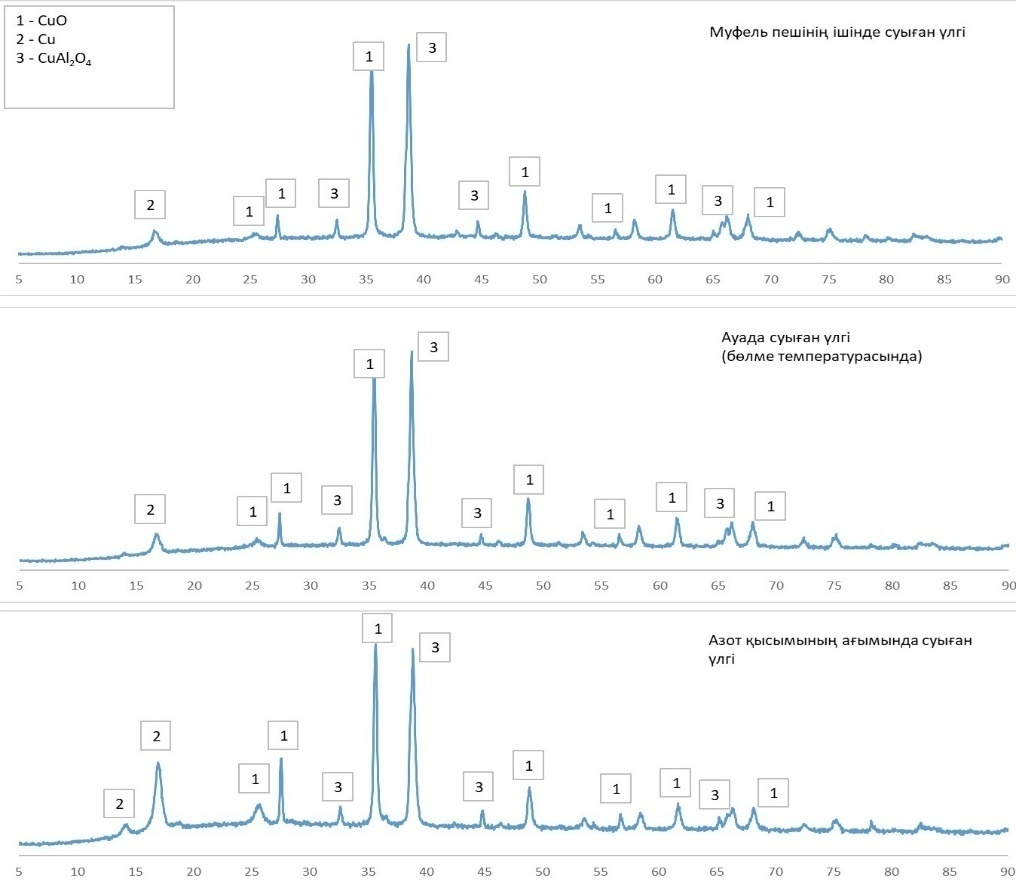
\includegraphics[width=0.6\textwidth]{assets/70}
	\caption*{2-сурет - Әртүрлі жағдайларда салқындатылғаннан кейінгі Al-Cu-O катализаторлар сериясының рентгендік құрылымдық спектрлері}
\end{figure}

\begin{figure}[H]
    \centering
    \begin{subfigure}[b]{0.32\textwidth}
        \centering
        
\includegraphics[width=\textwidth]{assets/71}
        \caption*{a)}
    \end{subfigure}
    \hfill
    \begin{subfigure}[b]{0.32\textwidth}
        \centering
        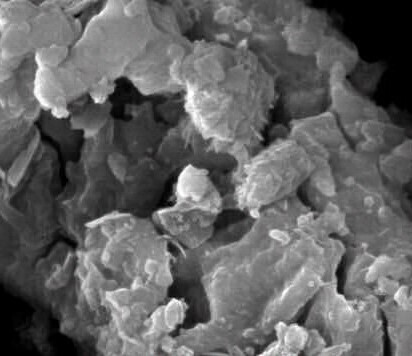
\includegraphics[width=\textwidth]{assets/72}
        \caption*{ә)}
    \end{subfigure}
    \begin{subfigure}[b]{0.32\textwidth}
        \centering
        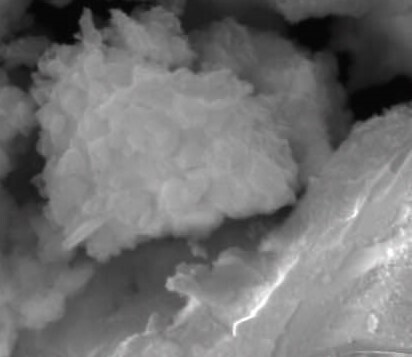
\includegraphics[width=\textwidth]{assets/73}
        \caption*{б)}
    \end{subfigure}
    \caption*{3-сурет - SHS жануынан кейінгі әртүрлі жағдайларда салқындатқаннан кейінгі Сu-Al-O катализаторлар сериясының сыну бетінің сканерлеуші электронды микрографтары: а) 700°C дейін қыздырылған муфель пешінің ішінде салқындатылған, ә) ашық ауада (бөлме температурасында) салқындатылған, б) азот қысымының ағынында салқындатылған үлгілер}
\end{figure}

\begin{multicols}{2}
Алынған катализаторлардың сапалық құрамы ұқсас болды, бірақ фазалық
қатынасы бойынша әр түрлі екенін байқадық. Фазалар арасындағы шамаланған
қатынастар рентген сәулесінің салыстырмалы қарқындылығы арқылы
анықталды.

Бастапқы СuO мен Al SHS жануына негізделіп жүргізілген тәжірибелер
(біркелкі бастау үшін өте аз мөлшерде Mg қосылған) де физика-химиялық
қасиеттер мен каталитикалық белсенділіктің салқындату жағдайларына
тәуелділігін көрсетті. Материалдардың сканерлеуші электронды
микроскопиясы негізгі себептердің біркелкі емес салқындатумен,
сондай-ақ, материалдың бетіне жақын жерде микрожарықтардың пайда болуына
және таралуына әкелетін салқындату кезіндегі термиялық соққымен
байланысты болуы мүмкін екенін көрсетті. Суығаннан кейінгі
катализатордың қысу беріктігінің міндері айтылған тұжырымдамалардың
жақсы көрсеткіші болып табылады. Азот ағынында салқындатылғаннан кейін
(үлгінің бетіндегі максималды салқындату жылдамдығына ие) өлшенген
беріктік шамамен 24МПа болды. SHS синтезінен кейін бөлме
температурасындағы ауада салқындатылған және 700°C температуралы пеште
салқындатылған материалдардың қысымға беріктігі сәйкесінше 17МПа және
11МПа дейін баяу азайды. Бұл сканерлеуші электронды микроскопия әдісімен
жасалған талдаулардың нәтижелерінен байқалатын микроқұрылымның өзгеруіне
байланысты болуы мүмкін деген тұжырымға келдік (3-сурет). Бұл бақылаулар
пештің ішіндегі температурада суыту шыны тәрізді фазаны төмендететінін,
атомдық диффузия арқылы кристалдануға ықпал ететінін көрсетеді, бұл
үлгінің жақсы адгезиясына және жоғары беріктігіне әкеледі. Дегенмен,
пештің ішінде ұзақ уақыт ұстау кристалдық бөлшектердің өсуіне әкеледі де
қысым беріктігін төмендетеді.

Синтезделген Cu-Al-O катализаторларының каталитикалық белсенділігі бөлме
температурасындағы ауада, азот ағынының астында, сондай-ақ, 700°C дейін
қыздырылған пеште салқындатылғаннан кейін зерттелді. Пеште салқындату
каталитикалық белсенділікті айтарлықтай төмендететіні анықталды. Осыған
дейін қарастырылған СЭМ бақылаулары бұл заңдылық микроқұрылымның
өзгеруінен, әсіресе дәндердің дамуы мен кристалдануынан туындауынан
болуы мүмкін екендігін көрсетті. Ауада және азот ағынының астында
(4-сурет) қатаю микроқұрылымның дамуын тоқтатады және кристалдану толық
емес болып шығады.
\end{multicols}

\begin{figure}[H]
	\centering
	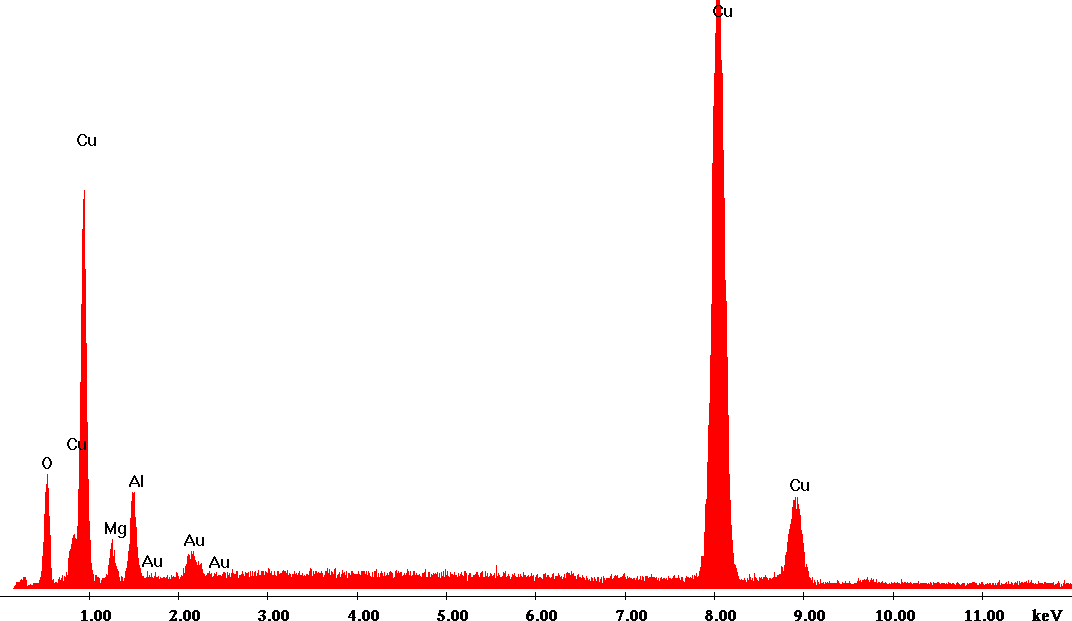
\includegraphics[width=0.8\textwidth]{assets/74}
	\caption*{4-сурет - Азот ағынында суытылған катализатордың элементтік құрамы}
\end{figure}

\begin{multicols}{2}
Екінші жағынан, SНS реакциясынан кейін пеште ұзақ уақыт ұстап салқындату
микроқұрылымның толық дамуына мүмкіндік береді және «дәндердің» дамуы
мен өсуіне мүмкіндік береді. Жылдам салқындату ақаулы құрылымның пайда
болуына әкелуі мүмкін және бұл ақаулар белсенділіктің негізі болады да,
катализатордың белсенді орталықтары ретінде әрекет етеді. Дегенмен, бұл
микроқұрылымдық деңгеймен теңестіріледі, сондықтан белгілі бір процестің
белсенділігі максималды болатын оңтайлы салқындату жылдамдығы болуы
керек. Сонымен қатар, ұзақ уақыт бойы қызып тұрған пештің ішінде суыту
микротор немесе интерфейстер арқылы атомдардың диффузиясына ықпал етіп,
«ақаулардың» концентрациясын төмендетеді. 5 және 6-суреттерде
көрсетілген нәтижелерді ескере отырып, SНS синтезінен кейін
катализаторды оңтайлы салқындату жылдамдығы -- азот ағынының астында
салқындату екені анықталды.
\end{multicols}

\begin{figure}[H]
	\centering
	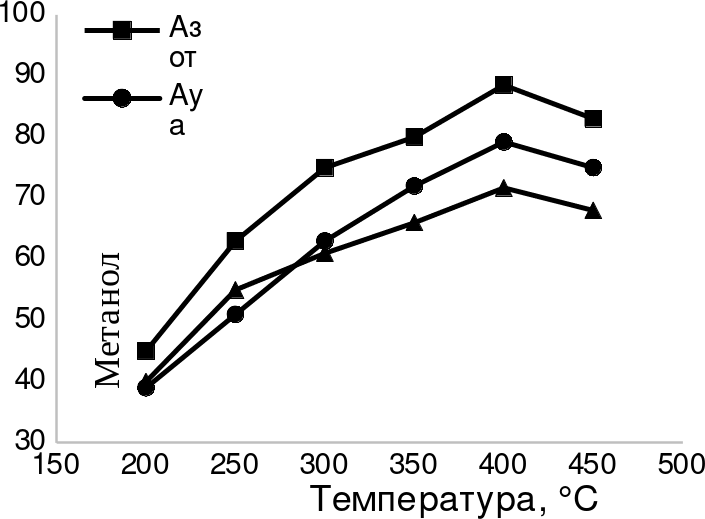
\includegraphics[width=0.5\textwidth]{assets/74.1}
	\caption*{5-сурет - Әртүрлі жағдайларда салқындағаннан кейін бірдей Сu-Al-O катализаторы үшін температураға байланысты метанолдың конверсиясы}
\end{figure}

5-суретте көрініп тұрғандай катализаторды салқындату жылдамдығы артқан
сайын, метанолдың конверсиясы да арта түседі. Ерекше атап өтетін жайт --
конверсия температурасының төмен болуы.

\begin{figure}[H]
	\centering
	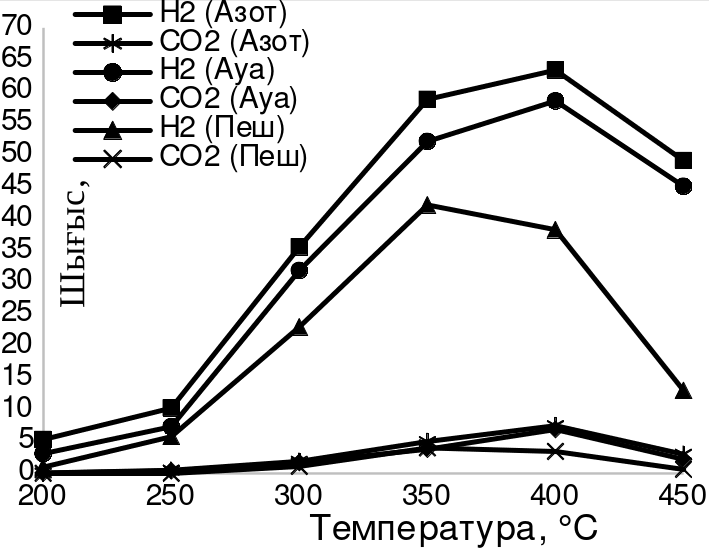
\includegraphics[width=0.5\textwidth]{assets/74.2}
	\caption*{6-сурет - Әртүрлі жағдайларда салқындағаннан кейін бірдей Сu-Al-O катализаторы үшін температураға байланысты Н\textsubscript{2} мен СО\textsubscript{2} шығымы}
\end{figure}

\begin{multicols}{2}
Осылайша, метанолдың каталитикалық риформинг процесі арқылы сутегі мен
көміртегінің қос тотығына дейін конверсиялану реакциясының оңтайлы
шарттары анықталды: T=400, Р=0,27 бар, V=100 мкл\textbackslash мин,
шикізат пен энергияны ұтымды тұтыну кезінде өнімнің максималды
шығымдылығын алу үшін, реакция қоспасындағы заттардың қатынасы
CH\textsubscript{3}OH:H\textsubscript{2}O=2,5:1 болды.

{\bfseries Қорытынды.} Осылайша, өздігінен таралатын жоғары температуралық
(SНS) синтезінен кейінгі үлгілерді салқындату мен суыту жағдайлары
катализаторлардың физикалық қасиеттері мен каталитикалық белсенділігіне
айтарлықтай әсер етеді. Жүйеге байланысты салқындату жылдамдығының
өзгеруі SНS катализаторларының құрамын да, құрылымын да өзгерте алады.
Әр түрлі салқындату жағдайларын қолдана отырып жүргізілген тәжірибелер
метанолдың сутегіге дейін конверсиялану процесінің каталитикалық
белсенділігі арту үшін оңтайлы салқындату жағдайлары мен жылдамдығы бар
екенін көрсетті. Бұл құбылыстың негізгі механизмдері құрамның,
микроқұрылымның және ақаулардың концентрациясының өзгеруіне байланысты
екені белгілі болды. Осы зерттеудің нәтижелері SНS катализаторларының
репродуктивтілігін, қасиеттерін және каталитикалық белсенділігін
жылдамдық пен салқындату жағдайларын бақылау арқылы арттыруға болатынын
растайды.

\emph{{\bfseries Қаржыландыру.} Зерттеу Қазақстан Республикасы ғылым және
жоғары білім министрлігінің қаржылық қолдауымен орындалды (AP19677006).}
\end{multicols}

\begin{center}
{\bfseries Әдебиеттер}
\end{center}

\begin{noparindent}
1. Vekinis G., Xanthoulou G. An overview of some environmental
applications of sefl-propagating high-temperature synthesis.// Advances
in environmental research. -2001.-Vol. 5(2). -P.117-128. DOI

10.1016/S1093-0191(00)00048-.

2. Peizhong F., Xuanhui Q., Farid A., Islam S.H. Self-propagating high
temperature synthesis of MoSi2 matrix composites// Rare metals.-
2006.-Vol. 25(3).- P. 225-230.

DOI 10.1016/S1001-0521(06)60044-2

3. Wang C., Yu F., Zhu M., Tang C., Zhang K., Zhao D., Dong L., Dai B.
(2019) Highly selective catalytic reduction of NOx by MnOx--CeO2--Al2O3
catalysts prepared by self-propagating high - temperature
synthesis // Journal of Environmental Sciences.-2019.-Vol.75.- P.124-135.

DOI 10.1016/j.jes.2018.03.011

4. Aghajanyan N.N., Dolukhanyan S.K., Ter-Galstyan O.P., Muradyan G.N.,
Hovhannisyan A.A. Self-propagating high-temperature synthesis of MAX
phases in Ti-Zr-Al-C system.//Ceramics international.-2023.-
Vol.49(14):24165-24170.-P. 24165-24170

DOI 10.1016/j.ceramint.2022.11.041.

5. Sanches-Rodriguez D., Yamaguchi S., Ihara D., Yamaura H., Yahiro H.
(2017) Self-propagating high-temperature synthesis of highly dispersed
noble metals on ceria powder: Application to Pd/CeO2~catalyst //Ceramics
International. -2017.- Vol. 43(16). -P.14533-14536.

DOI 10.1016/j.ceramint.2017.07.208

6. Hos T., Sror G., Herskowitz M. Autothermal reforming of methanol for
on-board hydrogen production in marine vehicles//International journal
of hydrogen energy.-2024.-Vol. 49.- P.

1121-1132. DOI 10.1016/j.ijhydene.2023.08.315.

7. Cubeiro M.L., Fierro J.L.G. Partial oxidation of methanol over
supported palladium catalysts// Applied Catalysis A: General.-1998.-
Vol. 168(2).- P. 307-322.

DOI 10.1016/S0926-860X(97)00361-X

8. Kang J., Song Y., Kim T., Kim S. Recent trends in the development of
reactor systems for hydrogen production via methanol steam reforming
//International journal of hydrogen energy. -2022.-Vol. 47. -
P.3587-3610. DOI 10.1016/j.ijhydene.2021.11.041.

9. Xanthopouou G., Vekinis G. Deep oxidation of methane using catalysts
and carriers produced by self-propagating high-temperature
synthesis//Applied Catalysis A: General.// -2000.- Vol. 199(2). -
P.227-238. DOI 10.1016/S0926-860X(99)00562-1

10. Hirano T., Purwanto H., Watanabe T., Akiyama T. Self-propagating
high-temperature synthesis of Sr-doped LaMnO3 perovskite as oxidation
catalyst//Journal of Alloys and Compounds.-2007.-Vol. 441. -- P.
263-266. DOI 10.1016/j.jallcom.2006.09.093

11. Guan B., Lin H., Zhan R., Huang Z. Catalytic combustion of soot over
Cu, Mn substitution CeZrO2-δ nanocomposites catalysts prepared by
self-propagating high-temperature synthesis method//Chemical Engineering
Science.-2018.- Vol. 189. -- P. 320-339.

DOI 10.1016/j.ces.2018.05.063
\end{noparindent}

\emph{{\bfseries Авторлар туралы мәліметтер}}

\begin{noparindent}
Асылбеков Е.Б. - т.ғ. магистрі, әл-Фараби атындағы Қазақ Ұлттық
университетінің PhD докторанты, Д.В. Сокольский атындағы «Жанармай,
катализ және электрохимия институты» АҚ, тотығу катализі зертханасының
ғылыми қызметкері, Алматы, Қазақстан, е-mail: yer-asyl@mail.ru;

Тунгатарова С.А. - х.ғ. докторы, профессор, Д.В. Сокольский атындағы
«Жанармай, катализ және электрохимия институты» АҚ, тотығу катализі
зертханасының меңгерушісі,; әл-Фараби атындағы Қазақ Ұлттық
университетінің профессоры, Алматы, Қазақстан, е-mail:
tungatarova58@mail.ru;

Xanthopoulou G.G. - х.ғ. докторы, профессор, наноғылым және
нанотехнология институты, Демокритос ҒЗҰО, Афины, Грекия, е-mail:
g.xanthopoulou@inn.demokritos.gr;

Байжұманова Т.С. - х.ғ. кандидаты, Д.В. Сокольский атындағы «Жанармай,
катализ және электрохимия институты» АҚ, тотығу катализі зертханасының
жетекші ғылыми қызметкері, Алматы, Қазақстан, е-mail: baizhuma@mail.ru;

Жұмабек М. - PhD, Д.В. Сокольский атындағы «Жанармай, катализ және
электрохимия институты» АҚ, тотығу катализі зертханасының аға ғылыми
қызметкері, Алматы, Қазақстан, е-mail:

manapkhan\_86@mail.ru.
\end{noparindent}

\emph{{\bfseries Information about authors}}

\begin{noparindent}
Assylbekov Y.B. {\bfseries -} PhD student of Al-Farabi Kazakh National
University, research associate of Laboratory of Oxidative Catalysis, JSC
``D.V. Sokolsky Institute of Fuel, Catalysis and Electrochemistry'',
Almaty, Kazakhstan, e-mail: yer-asyl@mail.ru;

Tungatarova S.A. - Doctor of Chemical Sciences, Professor, Head of the
Laboratory of Oxidative Catalysis, JSC ``D.V. Sokolsky Institute of
Fuel, Catalysis and Electrochemistry'', Professor of Al-Farabi Kazakh
National University, Almaty, Kazakhstan, e-mail: tungatarova58@mail.ru;

Xanthopoulou G.G. - Doctor of Chemical Sciences, Professor, Institute of
Nanoscience and Nanotechnology, NCSR Demokritos, Athens, Greece,
g.xanthopoulou@inn.demokritos.gr;

Baizhumanova T.S. - Leading Researcher, Candidate of Chemical Sciences,
Laboratory of Oxidative Catalysis, JSC ``D.V. Sokolsky Institute of
Fuel, Catalysis and Electrochemistry'', Almaty, Kazakhstan, e-mail:
baizhuma@mail.ru;

Zhumabek M. - PhD Doctoral student, Satbayev University; Researcher of
the Laboratory of Oxidative Catalysis, JSC ``D.V. Sokolsky Institute of
Fuel, Catalysis and Electrochemistry'', Almaty, Kazakhstan, e-mail:
manapkhan\_86@mail.ru.
\end{noparindent}
